When dealing with microfluidics, some important concepts should be kept in mind. The liquid flow should be kept as smooth as possible and be devoid of any flaws such as cross-current, eddies, swirls, or bubbles. In fluid dynamics, such a smooth flow state is called laminar flow and is characterized by an orderly movement of the particles within the liquid \cite{lagerstrom1996laminar,bruus2011theoretical}. The particles in that state move in straight lines parallel to the adjacent walls, and no mixing is observed between the flow layers. The reciprocal of laminar flow is called turbulent flow, and is observed at higher fluid speed and density, lower liquid viscosity, and for larger diameters of conduits (see \autoref{fig:LaminarTurbulent}. An important concept when defining the smoothness of a liquid flow is the Reynolds number. It is a dimensionless parameter that operates on the ratio of the inertial force to the shearing force of the flowing liquid. Its specific calculation depends on the geometry of the canal. For high Reynolds number, the flow is defined as turbulent, whereas it is defined as laminar for low Reynolds number \cite{lagerstrom1996laminar,bruus2011theoretical}. The density and viscosity of the liquid are parameters that are application specific, but the speed of the liquid and the diameters of the conduits are parameters that can be modified when designing a microfluidic sensor. Lower liquid velocity and smaller conduits should then be used to obtain a smooth laminar flow. \par
\begin{figure}[h]
    \centering
    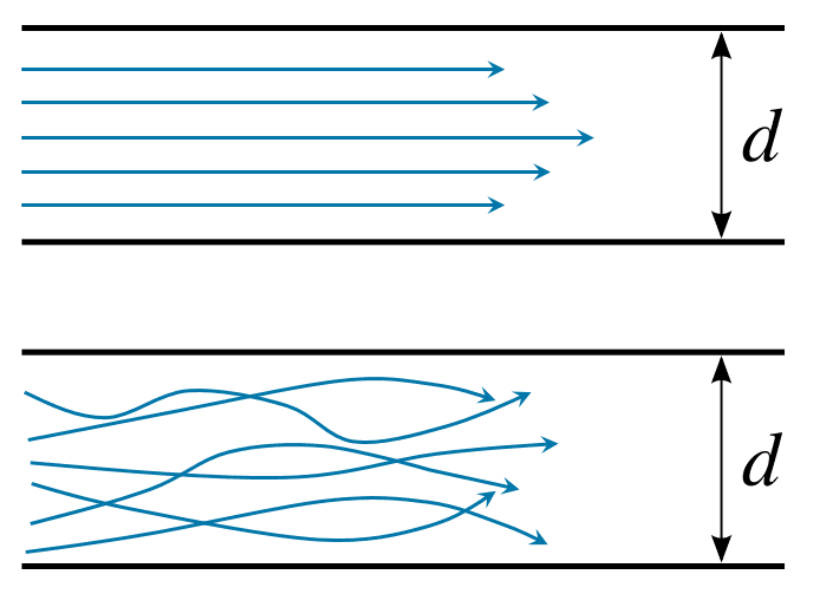
\includegraphics[width=0.5\textwidth]{LaminarTurbulent}
    \caption{Behavior of laminar [up] and turbulent [down] flow in a fluidic channel. \citep{simscale_2021}}
    \label{fig:LaminarTurbulent}
\end{figure}
The behaviors observed in microfluidics is analogous to those observed in electrical circuits: the current flow can be associated with the electrical current, the applied pressure with an applied ideal voltage source, and the resistance to the flow with the electrical resistance. Flow compliance, the analog of electrical capacitance, is also defined as the modification of the channel volume when an increase in pressure is observed \cite{bruus2011theoretical}. This generally happens for soft wall materials or when gas is compressed in the channel. Flow resistors are an important design consideration and can be adjusted by modifying the cross-section geometry and width, and length of the channel \cite{bruus2011theoretical,Olanrewaju2018}. \par

The capillary pressure is also affected by the geometry of the channel, meaning that such a variation is always associated with a decrease in flow rate and in flow speed (for $h<<w$, the flow rate is reduced in $\frac{1}{h^2}$ and the flow speed in $\frac{1}{h}$ \cite{lagerstrom1996laminar,bruus2011theoretical}. The flow rate follows a Poiseuille-Flow for low Reynolds number and laminar flow when applied with a pressure difference $\Delta P$ between its inlet and outlet, which is a parabolic fluid velocity across the circular channel cross-section, with a maximum velocity at the center and null-speed near the walls. To calculate the flow rate $Q$ in a microfluidic system, it is necessary to solve the Stockes equation, which can be rendered geometry independent using the flow resistor as a parameter \cite{bruus2011theoretical,Zimmermann2007}: 
\begin{equation}
   Q = \frac{1}{\nu} \frac{\Delta P}{R_f}
\end{equation}
Where $\nu$ is the viscosity of the liquid, $\Delta P$ the difference in pressure inside and in front of the liquid, and $R_f$ the total resistance to flow. It is important to note that since the flow rate depends on the viscosity, the flow resistance will increase as the gas present in the channel at the beginning is replaced by a liquid \cite{bruus2011theoretical,Zimmermann2007}. \par

The pressure difference in the microchannel $\Delta P$ can be created using capillary pump based on the Young-Laplace equation. Such pumps can however only hold nanoliters of liquid and induce flow rates in the nanoliters per seconds, meaning they are more suitable for immunoassay analysis than for long-term tests. These pumps are created using intricate channel geometries that maximize the pressure difference. This is often done by maximizing the liquid contact regions with the channels walls and by reducing the width and height of the conduits, such as in “tree lines”, “hexagons”, and “balled lines” geometries \cite{bruus2011theoretical,Zimmermann2007}. \par

Syringes are often used in microfluidics application despite some shortcomings. They create a pressure difference between the inlet and outlet, which is associated to a flow rate flow, flow resistance, and compliance of the channel \cite{SyringePumps,bruus2011theoretical}. The soft material generally used in microfluidics, such as the tubing made from Tygon, channel made in PDMS, plastic syringes, etc. get deformed when confronted to a pressure difference, which induces a compliance in the channel. This compliance, when associated to the channel resistance, creates a settling time analogous to the settling times of RC systems in electronics. This means that the systems lose in responsiveness when using syringe pumps, with the flow rate linearly increasing over a settling time after a pressure change is applied. The experiments using syringe pumps thus lose in responsiveness and reproducibility compared to those using more advanced microfluidic pressure controller \cite{SyringePumps,Olanrewaju2018,bruus2011theoretical}. \par

The wettability of surfaces is an important parameter in microfluidic applications since it governs the contact angle between the surface and the liquid. A surface is considered wettable in theory when the contact angle is less than 90° \cite{Olanrewaju2018}. Wettable surfaces, also call hydrophilic surfaces, generate a concave interface between liquid and gas, with a negative capillary pressure that sucks liquids inside the channel. Hydrophobic surfaces, on the other hand, are defined for contact angles higher than 90°. They create a convex interface between liquid and gas, and a positive pressure which pushes liquid out of the channel. These interactions are depicted in \autoref{fig:Surface_Wettability}. It is important to note that these liquid-solid interfaces are unaffected by gravity since surface forces are dominant compared to inertial forces in capillary channels. In practice, imperfections in the conduit can drastically modify the wettability and capillary pressure inside the channel, which can disrupt the channel’s functionality. Contact angles below 60° are thus chosen for adequate flowing and since contact angles close to 90° are associated with high capillary pressures which block the liquid flow [41]. This relation can be expressed by the Young-Laplace equation \cite{Olanrewaju2018,bruus2011theoretical}:
\begin{figure}[h]
    \centering
    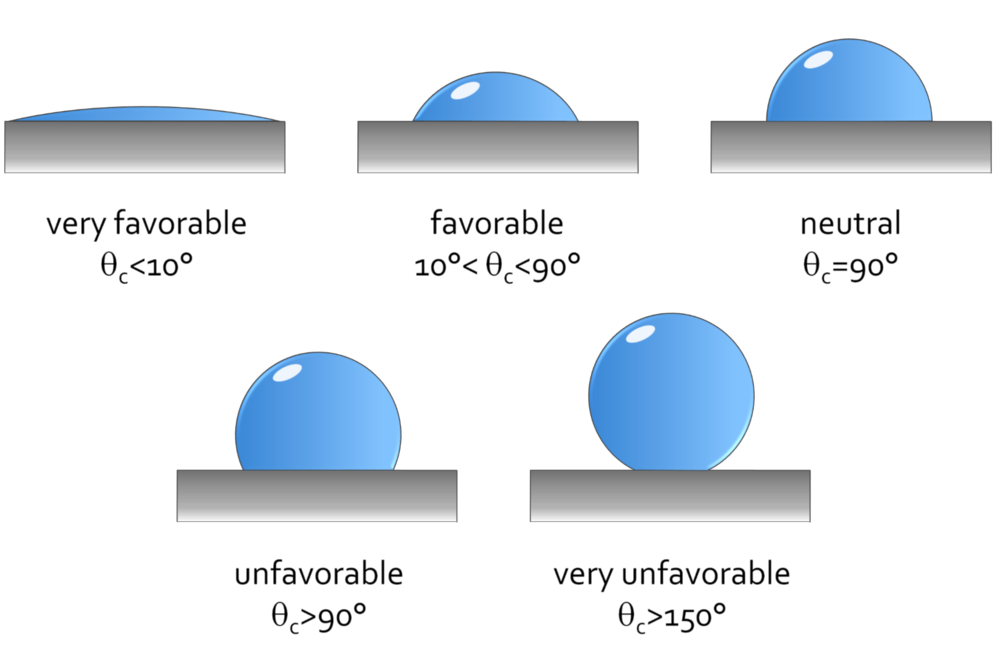
\includegraphics[width=0.8\textwidth]{Surface_Wettability}
    \caption{A droplet tend to cling to wettable surfaces, whereas it rolls off unwettable ones. \citep{surfacewettability}}
    \label{fig:Surface_Wettability}
\end{figure}
\begin{equation}
   \Delta P = -\gamma [\frac{cos(\theta_t)+cos(\theta_b)}{h} + \frac{cos(\theta_l)+cos(\theta_r)}{w}]
\end{equation}
where $\Delta P$ is the capillary pressure, $\gamma$ is the surface tension of liquid in the microchannel, $h$ and $w$ are the channel height and width respectively, and $\theta_t$, $\theta_b$, $\theta_l$, $\theta_r$ are the top, bottom, left, and right contact angles of liquid with the corresponding four microchannel walls \cite{Olanrewaju2018,bruus2011theoretical}. \par

Having contact angles lower than 60° on all walls often proves to be a challenging task since microchannels are generally made from heterogeneous materials. A sealing layer is often used, which features different fluidic properties than the rest of the conduit. The aspect ratio between $h$ and $w$ must then be chosen carefully as to not block the liquid flow when a hydrophobic material is used \cite{Olanrewaju2018}.\par

Additionally, the contact angle should always be kept higher than 30° to reduce the impacts of corner flow, which happens when a liquid flows between two surfaces with different contact angles. The liquid on the side of the most hydrophilic wall will precede the bulk flow. This may create deviations to the pressure predicted with the Young-Laplace equation and affect the uniform wetting of sensor electrodes \cite{Olanrewaju2018}. \par

Glass and silicon dioxides, two materials of choice for lithography-based microfluidic systems, have contact angles of 25° and 52°, respectively, making them both hydrophilic. PDMS, the leading substrate for quick prototyping, is, on the other hand, hydrophobic with a contact angle of 107° \cite{Olanrewaju2018,Trantidou2017}. Surface treatment is thus necessary to render it sufficiently wettable for use in capillary microchannels. The most common way to wet a surface is by exposing it to highly reactive plasma, ozone, or UV light \cite{Ufluidix}. High energy radicals are thus created and oxidize the surface, increasing its wettability. However, such treatments only modify the surface for a short while: 10min in the case of plasma. \citep{Trantidou2017} grafted silanes such as polyethylene glycol (PEG) or Polyvinyl alcohol (PVA) with hydrophilic end groups unto the PDMS surface after plasma treatment via heat immobilization to stabilize the surface wettability up to 30 days, with contact angles staying between 30° and 60°\cite{Olanrewaju2018,Ufluidix,Trantidou2017}. 